\documentclass{report}
\usepackage{float}

% depricated
\title{
	\iffalse
	\begin{tikzpicture}[remember picture,overlay]
		\node[anchor=north west,yshift=-5pt,xshift=-200pt]%
		at (current page.north east)
		{
\includegraphics[height=30mm]{images/unitn-logo}};
	\end{tikzpicture}
	\huge 
	\fi
	FixMi \\
	Analisi dei Requisiti
}
\author{Giovanni Santini, Riginel Ungureanu, Valerio Asaro}
\date{Anno accademico 2023/2024}

% for the image in the title
\usepackage{tikz}

% custom spacing
\usepackage{setspace}
\onehalfspacing

% footer and header
\usepackage{fancyhdr}
% \setlength{\headheight}{15.2pt}

% Table of contents link to corresponding sections
\usepackage{hyperref}
\hypersetup{
	colorlinks,
	citecolor=black,
	filecolor=black,
	linkcolor=black,
	urlcolor=black
}

% Remove che "Chapter" string before chapters
\iffalse
\makeatletter
\def\@makechapterhead#1{%
	\vspace*{50\p@}%
	{\parindent \z@ \raggedright \normalfont
		\interlinepenalty\@M
		\Huge\bfseries  \thechapter.\quad #1\par\nobreak
		\vskip 40\p@
}}
\makeatother
\fi

% Fancy chapters
\usepackage[Bjarne]{fncychap}
% options: Sonny, Lenny, Glenn, Conny, Rejne, Bjarne, Bjornstrup

%glossario
% \usepackage{glossaries}

\begin{document}


%title page
\begin{titlepage}
	\begin{figure}[t]
		\centering
\includegraphics[width=0.3\textwidth]{images/unitn-logo}
	\end{figure}
	\begin{center}
		\textsc{ \LARGE{Università degli Studi di Trento \\}}
		\textsc{ \LARGE{Facoltà di Informatica\\ }}
		\textnormal{ \LARGE{Corso di Ingegneria del Software\\}}
		\vspace{30mm}
		\fontsize{10mm}{7mm}\selectfont 
		\textup{FixMi \\ Analisi dei Requisiti}\\
	\end{center}
	
	\vspace{25mm}
	
	\centering
	\large Gruppo G43:\\ Giovanni Santini \\ Riginel Ungureanu \\ Valerio Asaro
	
	\vspace{20mm}
	
	\centering{\large{Anno Accademico 2023/2024 \\ Trento }}
	
\end{titlepage}


% use header and footers
\pagestyle{fancy}
\fancyhead[R]{\chaptername\ \thechapter}  % header

%\maketitle
\tableofcontents
\newpage





\section{Scopo del documento}
Il seguente documento riporta la definizione e l'analisi del progetto "FixMi" in linguaggio naturale.
In particolare il documento mira a:

\begin{enumerate}
		
	\item Stabilire gli obiettivi del progetto.
	\item Definire i requisiti funzionali e non funzionali.
	\item Presentare i requisiti di Front-End del progetto.
	\item Presentare i requisiti di Back-End del progetto.
	\item Stabilire ruoli e funzioni dei singoli membri del team di sviluppo.
	\item Definire tecniche e strumenti utili alla realizzazione del progetto.

\end{enumerate}


\section{Informazioni del Documento}

% table
\begin{center} % center the table
	\centering
	\begin{tabular}{ |p{4cm}|p{4cm}|  }
		\hline
		\centering Campo & \qquad\qquad Valore \\ % I found no other way...
		\hline
		Titolo del Documento & Analisi dei Requisiti \\
		\hline
		Titolo del Progetto & FixMi \\
		\hline
		Autori del Documento &
		Giovanni Santini \\ & Riginel Ungureanu \\ & Valerio Asaro \\
		\hline
		Responsabile del Progetto & Riginel Ungureanu\\
		\hline
		Versione del documento & 1.3 \\
		\hline
	\end{tabular}
\end{center}


\chapter{Obiettivo del progetto}


Di seguito vengono illustrati in maniera discorsiva gli obiettivi principali e secondari del progetto in questione.

\section{Obiettivo Principale}

L’obiettivo del progetto è la realizzazione di una Web-App denominata "FixMi": un'applicazione web gestionale sviluppata per un negozio di articoli informatici ed elettronici. Tale software svolgerà il ruolo di supporto all’attività di commercio e riparazione dei dispositivi elettronici mettendo in comunicazione datore di lavoro, dipendenti e clienti.


\section{Obiettivi Secondari}

Successivamente vengono elencati gli obiettivi secondari del progetto, numerati tramite acronimo "OSx" (Obiettivi Secondari), dove x è il numero che identifica inequivocabilmente un obiettivo da un altro. Questi obiettivi estendono quello principale e non sono da considerare di minore importanza durante l’analisi dei requisiti.


\subsection*{OS1 Autenticazione}
L’applicazione dispone di un sistema di distinzione dei ruoli: "Manager", "Dipendente" e "Cliente". Il sistema permetterà diverse funzionalità in base al livello di autorizzazione di cui si dispone.


\subsection*{OS2 Magazzino}
Il sito fornisce ai dipendenti e al manager un sistema di gestione del magazzino con il quale si potrà aggiungere e rimuovere merce, oltre a controllarne la quantità disponibile.


\subsection*{OS3 Negozio}
Il sito offre ai clienti un negozio, il cui catalogo si interfaccia con il magazzino precedentemente descritto (OS2), che permetta loro di inserire degli articoli nel carrello e, successivamente, di effettuarne l'acquisto. I dipendenti potranno visualizzare e gestire gli ordini e le richieste di vendita effettuate dai clienti.


\subsection*{OS4 Riparazione}
L’applicazione offre ai clienti la possibilità di richiedere la riparazione di un proprio articolo, inoltre offre ai dipendenti la possibilità di organizzare l’attività di riparazione di tale articolo.


\subsection*{OS5 Assistenza}
Il sito presenta ai clienti la lista dei contatti aziendali, nonché la possibilità di inserire una richiesta di assistenza relativa al sito, un ordine o una riparazione. I dipendenti potranno gestire le richieste e comunicare direttamente con i clienti.


\subsection*{OS6 Feedback} 
Il sito dispone agli utenti un'area "feedback" in cui potranno inviare dei giudizi sulla qualità del servizio offertogli e dei suggerimenti su come migliorare ulteriormente quest'ultimo.

\subsection*{OS7 Gestione Dipendenti}

Il manager può gestire i profili di tutti i dipendenti, visualizzarne le statistiche e lo storico delle attività. Inoltre si affida al manager il compito di aggiungere, rimuovere e modificare i profili "Dipendente" nel corso del tempo dell'attività aziendale.


\subsection*{OS8 Gestione Task}
L’applicazione presenta ai dipendenti e al manager un sistema di gestione delle Task, ossia le varie attività che i dipendenti possono prendere in carico e devono completare. Il ruolo del manager prevede la supervisione delle Task.


\chapter{Requisiti}
Posto l’obiettivo del progetto segue la definizione dei requisiti del sistema, suddivisi in Requisiti Funzionali (RF) e Requisiti Non Funzionali (RNF).



\section{Requisiti Funzionali}
Segue la lista dei Requisiti Funzionali (RF) individuati per il progetto.


\subsection*{RF0 Requisiti Generali}
Il sito deve manifestare una distinzione esplicita tra i tre tipi di utente, ossia Cliente, Dipendente e Manager, ognuno con accesso a funzionalità e privilegi diversi.
In vista di questo, la seguente sezione verrà divisa in base al tipo di utente interessato.

\subsection{Utente}

\subsection*{RF1 Profilo}

Avere un profilo è il primo passo verso l'interazione con "FixMi". Nel momento in cui si crea il proprio profilo si passa dall'essere un "Utente" ad essere un "Cliente", ricevendo nuovi servizi e vantaggi. Di seguito una lista dei requisiti per la corretta implementazione del profilo all'interno del sito web.

\subsubsection*{RF1.1 Login}

Il sito deve presentare una pagina di login.

\begin{enumerate}
	\item La pagina deve mostrare due campi “e-mail” e “password” e un bottone "login".
	
	\item La procedura di accesso deve andare a buon fine se e solo se i campi "e-mail" e "password" inseriti corrispondono entrambi ad un profilo già registrato nel sistema.
	
	\item L'applicazione deve mostrare una nuova pagina di login ed un messaggio di errore qualora il login fallisse.
	
	\item L’utente deve essere in grado di raggiungere la pagina di registrazione specificata in RF2 dalla pagina di login.
\end{enumerate}


\textbf{User Story:}
Come Utente, voglio poter effettuare il login nel mio profilo per accedere alle funzionalità dedicate.

	\subsubsection{RF1.2 2FA}
	La pagina deve implementare una tecnologia 2FA ("Two Factor Authentication") secondo le seguenti modalità:
	
	\begin{enumerate}
	\item L'applicazione deve generare un codice OTP ("One-Time Password") sul momento e inviarlo all'utente attraverso la e-mail inserita.
	
	\item 	La pagina deve chiedere l'inserimento del codice appena generato per continuare con successo.
	
	\item Un codice OTP non deve essere più valido dopo minuti 5 dalla la sua generazione.
	
	\item L'applicazione deve dare la possibilità di generare un nuovo codice OTP, sovrascrivendo il codice precedente.

	\end{enumerate}
	
	\subsubsection*{RF1.3 Reimpostazione/Recupero Password}
	Il sito deve offrire la possibilità all'utente di recuperare la password nel caso in cui abbia dimenticato quella precedentemente associata al suo profilo:
	\begin{enumerate}
			
	\item Il sistema deve chiedere il campo "e-mail" associata al profilo di cui si vuole recuperare la password.
	\item L'applicazione deve implementare 2FA come specificato in RF1.2
	\item L'utente dovrà inserire una nuova password da associare al profilo.
	\item L'utente dovrà digitare la nuova password due volte per ridurre la probabilità di errori di battitura.
	\item La nuova password deve rispettare i vincoli specificati in RNF2.
	\item La procedura deve fallire qualora non vi esistesse alcun profilo associato alla e-mail inserita nell'omonimo campo.

	\end{enumerate}

\subsection*{RF2 Registrazione}
Il sito deve dare la possibilità ad un utente di registrarsi:
\begin{enumerate}
	\item La pagina deve rappresentare i campi "e-mail" e "password" (due volte). 
	\item La password deve essere conforme come specificato in RNF2.
\end{enumerate}

\subsubsection*{RF2.1 Verifica E-mail}
L'applicazione deve verificare la mail dell'utente per terminare la registrazione con successo:

\begin{enumerate}
	\item L'applicazione deve inviare un codice di 6 cifre, generato in maniera casuale sul momento, alla e-mail specificata dall’utente e mostrare un campo "inserisci codice".
		
	\item L'applicazione deve dare la possibilità all’utente di inviare un nuovo codice di verifica del profilo. Il codice precedente non deve essere più valido per completare la registrazione.
		
\end{enumerate}


\subsubsection*{RF2.2 Terminazione Registrazione}
\begin{enumerate}
	\item La registrazione deve terminare con successo, caricando automaticamente la pagina di login (RF1), qualora il codice inserito nel campo "inserisci codice" corrispondesse a quello inviato tramite e-mail, e i campi "e-mail" e "password" fossero validi.
	\item Se una delle condizioni del punto precedente non venisse soddisfatta, la registrazione non deve proseguire e la pagina deve permettere di effettuare modifiche ai dati inseriti nei campi.
	\item Il livello di permessi del nuovo profilo successivamente alla registrazione deve essere di tipo Cliente.
	\item La registrazione non deve terminare con successo se un utente tenta di registrarsi con una e-mail a cui è associato un profilo esistente.

\end{enumerate}


\subsection*{RF3 Negozio Utente}
Il sito deve presentare una pagina "Negozio”: 

\begin{enumerate}
	\item La pagina deve permettere di visualizzare gli oggetti presenti nel magazzino al momento del caricamento della stessa.
	
	\item L’utente deve essere in grado di ordinare gli oggetti per nome o per prezzo, ricercare una stringa tra i nomi degli oggetti nel negozio.
	
	\item Ogni oggetto deve avere una pagina dedicata.
\end{enumerate}


\subsection*{RF4 Informazioni / Contatti}
L’applicazione deve offrire all’utente una pagina dove sono visibili dati utili riguardo l'azienda:

\begin{enumerate}
	\item Descrizione dell'azienda.
	\item Una lista contenente varie "Frequently Asked Questions" (FAQ) riguardo il funzionamento del sito.
	\item Contatti dell’impresa: numeri di telefono, e-mail e indirizzo.
	\item Il sito deve mostrare inoltre un riquadro con una mappa dove è possibile visualizzare la posizione del negozio.
\end{enumerate}


\subsection{Cliente}
Il sito deve dare la possibilità al cliente di autenticarsi attraverso la pagina di login come specificato in RF1 inserendo le proprie credenziali (e-mail e password) inserite in fase di registrazione, in modo da poter accedere alle funzionalità elencate di seguito:

\subsubsection*{RF1.4 Cambio Password}
Il sito deve offrire la possibilità all'utente di cambiare password nel caso avesse già un profilo:
\begin{enumerate}
	
	\item Il sistema deve chiedere il campo "e-mail" associata al profilo di cui si vuole cambiare la password.
	\item L'applicazione deve implementare 2FA come specificato in RF1.2
	\item La nuova password dovrà essere digitata due volte per ridurre la probabilità di errori di battitura.
	\item La nuova password deve rispettare i vincoli specificati in RNF2.
	\item La procedura deve fallire qualora non vi esistesse alcun profilo associato alla e-mail inserita nell'omonimo campo.
	
\end{enumerate}

\subsubsection{RF1.5 Log Out}

L'applicazione deve dare la possibilità al cliente / dipendente / manager di uscire dal proprio profilo qualora fosse autenticato, rendendoli di conseguenza degli "utenti" (2.1.1)

\subsubsection{RF1.6 Eliminazione profilo}

L'applicazione deve dare la possibilità al cliente e ai dipendenti di potere cancellare il proprio profilo, con tutte le relative informazioni e i dati legati alla persona associata ad esso, da ogni tipo di memoria, base di dati o altro metodo di memorizzazione appartenenti all'applicazione "FixMi".

\begin{enumerate}
	\item Il sistema deve chiedere il campo "e-mail" associato al profilo che si vuole eliminare.
	\item L'applicazione deve implementare 2FA come specificato in RF1.2
	\item Viene richiesto l'inserimento della password legata al profilo una ultima volta prima della definitiva eliminazione.
	\item La procedura deve fallire qualora non vi esistesse alcun profilo associato alla e-mail inserita nell'omonimo campo.
\end{enumerate}
\subsection*{RF5 Negozio Cliente}
Il sito deve permettere al cliente, oltre alle funzionalità definite in RF3 per gli utenti, le seguenti funzionalità:

\subsubsection{RF5.1 Carrello}
Il sito deve avere una pagina dedicata al carrello del cliente.
Il sito deve permettere al cliente, nella pagina dedicata a un specifico articolo, di inserirlo nel proprio carrello.

\begin{enumerate}
	\item La pagina deve avere un elenco di tutti i prodotti che sono stati immessi nel carrello. Ogni prodotto contenuto in elenco deve mostrare il nome, il prezzo, una foto e un pulsante “Rimuovi”.
	
	\item La pagina deve permettere al cliente di rimuovere un elemento dal proprio carrello. % premendo il pulsante “Rimuovi” posizionato accanto ad ogni elemento.

	\item Ogni prodotto deve portare alla pagina dedicata allo stesso cliccando sul nome contenuto in elenco.
	
	\item La pagina deve mostrare il prezzo totale, ossia la somma dei prezzi degli elementi del carrello.

	\item La pagina deve avere un tasto “procedi al pagamento” con il quale si procede alla pagina di pagamento specificata sotto.
	
	\item L'utente deve avere la possibilità di vedere i prodotti salvati nel proprio carrello anche dopo aver chiuso la pagina.

\end{enumerate}

\subsubsection*{RF5.2 Pagamento}
La pagina deve fornire diversi metodi di pagamento:

\begin{enumerate}

	\item La pagina deve fornire il pagamento tramite "Paypal" e "Bancomat" con circuiti "Visa" e "Mastercard".

	\item Una volta effettuato il pagamento con successo, il sito deve fornire un riepilogo dell’acquisto e un messaggio che invita il cliente a recarsi in negozio per il ritiro dei prodotti.
	\item Il sito deve creare per i dipendenti una Task “magazzino” (RF9), dettagliando i prodotti richiesti.
	\item Il sito deve inviare i dettagli del pagamento al software di accounting scelto.
	\item Il sito deve eliminare gli elementi dal carrello dell’utente una volta effettuato il pagamento.
\end{enumerate}

\subsection*{RF6 Riparazione}

Il sito deve offrire al cliente la possibilità di inviare, compilando un apposito documento, una richiesta di riparazione per un proprio articolo di elettronica.
\begin{enumerate}


	\item Il documento deve richiedere i campi "nome", "cognome", "e-mail", "numero di telefono", "descrizione del problema" e opzionalmente "foto". Una volta compilato, il documento deve poter essere spedito attraverso un apposito bottone etichettato "Invia".
	
	\item L’applicazione deve generare una Task di tipo “riparazione” successivamente all’invio della richiesta da parte del cliente (il sistema di Task è specificato in RF9).
	
	\item Qualora il cliente abbia inviato una riparazione, il sito deve mostrare al cliente lo stato della propria riparazione in un'apposita pagina "stato riparazioni", interfacciandosi con il sistema di Task specificato in RF9. In caso non vi siano riparazioni, la pagina deve mostrare la scritta "Nessuna riparazione registrata".
	
\end{enumerate}

\subsection*{RF7 Assistenza}
Il sito deve permettere al cliente di richiedere assistenza e comunicare con l'azienda attraverso un modulo da compilare:

\begin{enumerate}
	\item Il modulo deve presentare i campi "e-mail", "descrizione richiesta" e un bottone "Invia".
	
	\item L’applicazione deve generare una Task di tipo “assistenza” successivamente all’invio della richiesta di assistenza da parte del cliente. Il sistema di Task è specificato in RF9.
	
	
\end{enumerate}

\subsection*{RF8 Feedback}
Il sito deve dare la possibilità al cliente di inviare anonimamente del feedback attraverso una pagina dedicata.
\begin{enumerate}
	\item La pagina deve contenere i campi "disponibilità azienda", "velocità riparazione", "soddisfazione riparazione", "soddisfazione sito web", "idee per migliorare" e un bottone "Invia".

	\item Il sito deve creare una Task assistenza con i contenuti dei campi inseriti dall'utente.

	
\end{enumerate}

\subsection{Dipendente}
Il sito deve dare la possibilità al dipendente di autenticarsi attraverso la pagina di login (RF1) inserendo le proprie credenziali (e-mail e password) fornitegli dal manager, in modo da poter accedere alle funzionalità dei clienti  e quelle riservate ai dipendenti elencate qui sotto.

\subsection*{RF9 Pagina Task}

Il sito deve offrire una pagina “Task” ai dipendenti autenticati, il sistema delle \textit{Task} è definito qui di seguito:

\subsubsection*{Definizione Task}

Una Task è un'attività sulla quale un dipendente o un manager può decidere di lavorare. Esistono diverse tipologie di Task, caratterizzate da una \textit{Task-Tag} ed una descrizione di massimo 200 caratteri.\\
Le Task possono essere in uno dei seguenti stati: 
\begin{itemize}
	\item Da eseguire
	\item In lavorazione
	\item In pausa
	\item Completata
	\item Fallita
\end{itemize}
Una \textit{Task-Tag} è una e una sola stringa tra le seguenti:
\begin{itemize}
	\item Magazzino
	\begin{itemize}
		\item Il dipendente accede alla pagina del magazzino (RF10) per apportare eventuali modifiche o visualizzare i vari articoli.
	\end{itemize}
	\item Negozio
	\begin{itemize}
		\item Il dipendente si assume il compito di rimanere alla cassa per interagire con eventuali clienti.
	\end{itemize}
	\item Assistenza
	\begin{itemize}
		\item Il dipendente visualizza la richiesta di supporto dal cliente tramite e-mail. Il dipendente potrà rispondere per e-mail al cliente in base alle esigenze del caso, secondo la propria discrezione.
	\end{itemize}
	\item Riparazione
	\begin{itemize}
		\item Il dipendente si assume il compito di rimanere alla cassa per interagire con eventuali clienti.
	\end{itemize}
\end{itemize}

\subsubsection*{Definizione Work-Tag}
Ad ogni profilo dipendente sono associate una o più \textit{Work-Tag}. Una \textit{Work-Tag} è una stringa dello stesso tipo di una \textit{Task-Tag}.\\
Ogni dipendente potrà lavorare solo sulle Task che hanno gli stessi o meno \textit{Task-Tag} rispetto ai \textit{Work-Tag} del dipendente.

\subsubsection*{RF9.1 Interagire con le Task}

Nella pagina "Task", il dipendente deve essere in grado di:

\begin{enumerate}
	\item Visualizzare la lista delle Task ed i corrispettivi \textit{Task-Tag} selezionate per il dipendente in base al suo corrispettivo \textit{Work-Tag}.
	
	\item Selezionare una Task dalla lista da eseguire o da quelle messe in pausa, contrassegnandola come in lavorazione, solo nel caso in cui il dipendente non presenti alcuna Task in lavorazione.
	
	\item Mettere in pausa la Task in esecuzione, la Task verrà contrassegnata come “In pausa” e il dipendente potrà selezionare una nuova Task dalla lista.
	
	\item Contrassegnare una Task come “completata”  insieme al nome del / dei dipendente/i responsabili del completamento e alla data, oppure come “fallita” nel caso ci fossero stati dei problemi. Il dipendente allora potrà scegliere una nuova Task dalla lista.
	
	\item Creare una nuova Task di qualsiasi tipologia, impostando \textit{Task-Tag} e la descrizione (anche vuota).
	
\end{enumerate}

\subsection*{RF10 Magazzino}
Il dipendente deve aver la possibilità di interagire con il magazzino in un'apposita pagina, in particolare:
\begin{enumerate}
	\item Visualizzare i prodotti all'interno del magazzino ordinati per nome o per data di arrivo, in modo crescente o decrescente.
	\item Aggiungere articoli.
	\item Rimuovere articoli.
\end{enumerate}

\subsection{Manager}
Il sito deve dare la possibilità al manager di potersi autenticare nella pagina di login, fornendo e-mail e password del profilo manager.

\subsection*{RF11}
Se un profilo è di tipo manager, deve poter accedere a tutte le funzionalità del profilo “dipendente” specificate sopra.

\subsubsection*{RF11.1 Gestione dei Dipendenti}
Il manager deve essere in grado di:

\begin{enumerate}
	
	\item Aggiungere profili “Dipendente” dall’applicazione inserendo l’e-mail del profilo in un apposito campo.
	\item Aggiungere dati Anagrafici associati all'account dipendente , "nome", "cognome", "data di nascita", "giorno assunzione".
	\item Rimuovere dipendenti selezionando la e-mail del dipendente e rimuovendola dalla lista dipendenti.
	
	\item Assegnare e rimuovere una o più \textit{Work-Tag} ai dipendenti. 
	
	\item Visualizzare informazioni dei dipendenti in apposita pagina, in particolare:
	
	\begin{itemize}
		\item Informazioni Biografiche.
		\item Storico con attività e record delle Task svolte / in svolgimento. Lo storico deve poter essere filtrato e ordinato tramite data di inizio e fine Task, nome dipendente, lista di Task-Tag.
		
	\end{itemize}
	
	\item Il profilo manager ha tutte le \textit{Work-Tag} assegnate per il proprio profilo.
		
\end{enumerate}

\subsubsection{RF11.2 Gestione delle Task}
Il manager deve essere in grado di:

\begin{enumerate}
	\item Creare una nuova task nel sistema.
	\item Visualizzare l'elenco di tutte le task nel sistema.
	\item Rimuovere tasks dal sistema.
\end{enumerate}

% table, da updateare
\begin{table}[h]
\begin{center} % center the table
	\centering
	\begin{tabular}{ |p{4cm}|p{4cm}|  }
		\hline
		\centering Obiettivi & \qquad\qquad Requisiti \\ % I found no other way...
		\hline
		OS1 Autenticazione & RF1, RF2 \\
		\hline
		OS2 Magazzino & RF9, RF10 \\
		\hline
		OS3 Negozio &
		RF3, RF9, RF10 \\
		\hline
		OS4 Riparazione & RF6, RF9\\
		\hline
		OS5 Assistenza & RF7, RF9 \\
		\hline
		OS6 Feedback & RF8, RF9 \\
		\hline
		OS7 Gestione dei Dipendenti & RF11 \\
		\hline
		OS8 Gestione Task & RF9, RF11.2 \\
		\hline
	\end{tabular}
\caption{Relazione tra Obiettivi e Requisiti Funzionali}
\end{center}
\end{table}

\pagebreak


\section{Requisiti Non Funzionali}
Di seguito vengono elencati i requisiti non funzionali dell’applicazione, numerati con acronimo "RNF".

\subsection*{RNF1 Intuitività e Accessibilità}
Il sito deve apparire semplice, sia sotto l'aspetto visivo che sotto l'aspetto pratico:
\begin{enumerate}
	\item In media l’utente deve essere in grado di capire le funzionalità con una sola lettura della descrizione.
	\item Il sito deve essere disponibile sia in lingua italiana che in lingua inglese, l’utente con un livello di lingua "A1" è in grado di leggere e comprendere il contenuto.
	\item Il sito deve avere un design consistente nella sua interezza, utilizzando un singolo font e una palette fissa di colori.
\end{enumerate}
\subsection*{RNF2 Sicurezza}
Il sito deve gestire ogni comunicazione in maniera sicura, sia tra utenti e server, che tra i servizi esterni di cui usufruisce:
\begin{enumerate}
	\item Il sito deve garantire che i dati sensibili siano crittografati e inaccessibili a soggetti indesiderati.
	\begin{itemize}
		\item Il sito deve utilizzare un algoritmo di hashing di tipo "SHA-3" per il controllo e la memorizzazione delle passwords.
		\item Il sito deve utilizzare i protocolli "tls" e "https" per ogni comunicazione tra utenti e servizi.
	\end{itemize}
	\item Il sito deve verificare l’identità dell’utente attraverso il 2FA come specificato nel RF1.
	\item Il sito deve, in fase di registrazione e di modifica password, controllare la sicurezza della password, ossia assicurarsi che la password  abbia almeno una lunghezza pari a 10 caratteri e presenti almeno un numero, una lettera maiuscola e un carattere speciale dalla lista \begin{verbatim} ! ? $ % ^ & * ( ) _ - + = { [ } ] : ; @ # | \ < , > . \end{verbatim}
\end{enumerate}


\subsection*{RNF3 Privacy}

L’applicativo deve essere conforme alle principali direttive sull’utilizzo e la gestione dei dati personali del cliente, del dipendente e del manager. In particolare il sito dovrà rispettare le normative del GDPR:
\newline Il GDPR (Regolamento Generale sulla Protezione dei Dati) è una legge europea che riguarda la protezione dei dati personali.
Le principali aree di focus del GDPR includono il consenso esplicito per la raccolta dei dati, la trasparenza nell'uso dei dati, la possibilità di accesso e cancellazione dei dati personali da parte dell'individuo, e misure di sicurezza per proteggere tali dati. 


\subsection*{RNF4 Affidabilità e Disponibilità}
\begin{enumerate}
	\item la probabilità che il sito fornisca i risultati desiderati senza interruzioni o tempi di inattività deve essere maggiore del 99\%
	\item la probabilità che il sito rimanga operativo in un determinato momento indipendentemente dal numero di guasti già subiti dal sistema deve essere maggiore del 99\%
	 
\end{enumerate}
\subsection*{RNF5 Performante}
Il sito deve offrire velocità di accesso ai servizi offerti in tempi rapidi:
\begin{enumerate}
	\item Il sito deve elaborare l'inserimento di un articolo nel magazzino in meno di un secondo.
	\item Il sito deve inviare le e-mail di 2FA(specificata in RF1) in meno di 5 secondi.
	\item Il sito deve aggiornare la lista delle Task (in caso di completamento, aggiunta, messa in pausa) in meno di un secondo.
\end{enumerate}

\subsection*{RNF6 Compatibilità e Portabilità}
L'applicazione deve essere supportata su una molteplice quantità di dispositivi.
Tra i principali vi sono:
\begin{enumerate}
	\item Dal lato client, computer e dispositivi mobili aventi un browser che supporta:
    \begin{itemize}
		\item html5
		\item https
		\item tls 1.2
	\end{itemize}
\end{enumerate}
Il sito deve essere "responsive", ossia deve potersi adattare alla dimensione degli schermi dei principali dispositivi in commercio, quali:
\begin{enumerate}
	\item TV e monitor di PC e Laptop 
	\begin{itemize}
		\item Aspect Ratio da 4:3, 16:9, 21:9
	\end{itemize}
	\item Smartphone
	\begin{itemize}
		\item Iphone X,XR,11,\dots , 14
		\item Tutti i modelli Xiaomi dal 2018 in poi 
		\item Tutti i modelli Samsung dal 2018 in poi
		\item Tutti i modelli Motorola dal 2018 in poi 
		\item Tutti i modelli Huawei dal 2018 in poi 
	\end{itemize}
	\item Tablet 
	\begin{itemize}
		\item Ipad Air, Pro dal 2018 in poi
		\item Tutti i modelli Xiaomi dal 2018 in poi
		\item Tutti i modelli Samsung dal 2018 in poi
	\end{itemize}
\end{enumerate}
\subsection*{RNF7 Mantenibilità e Scalabilità}
\begin{enumerate}
	\item Il sito, al fine di essere facilmente mantenibile, deve possedere un codice sorgente con le seguenti caratteristiche:
	\begin{itemize}
		\item Il codice sorgente del back-end deve essere modulare, utilizzando un'architettura a microservizi come descritto nel capitolo 3.2 - Design del back-end.
		\item Il codice sorgente deve rispettare le linee guida ufficiali del linguaggio scelto.
	
	\end{itemize} 
\end{enumerate}
\subsection*{RNF8 Conformità}
L'applicazione deve essere conforme alle normative di legge in materia di siti web imposti dall'Unione europea, inoltre vengono rispettati i seguenti:
\begin{enumerate}
	\item GDPR
	\item W3C WAI
\end{enumerate}
\chapter{Design}

\section{Design del Front-End}

In seguito vengono mostrate schermate delle principali aree di FixMi, essi rispecchiano le caratteristiche descritte dal (RF1) e vengono mostrate attraverso le tre tipologie di schermo discusse nel (RNF6). 

\subsection*{Schermata Login}

La schermata "Login" permette all'utente di inserire l'e-mail e la password del suo profilo ed in seguito di premere il bottone "ACCEDI", nel caso in cui l'utente non abbia ancora creato un proprio profilo egli potrà farlo accedendo all'area "Registrazione" attraverso il bottone "REGISTRATI".

\begin{figure}[H]
	\centering
	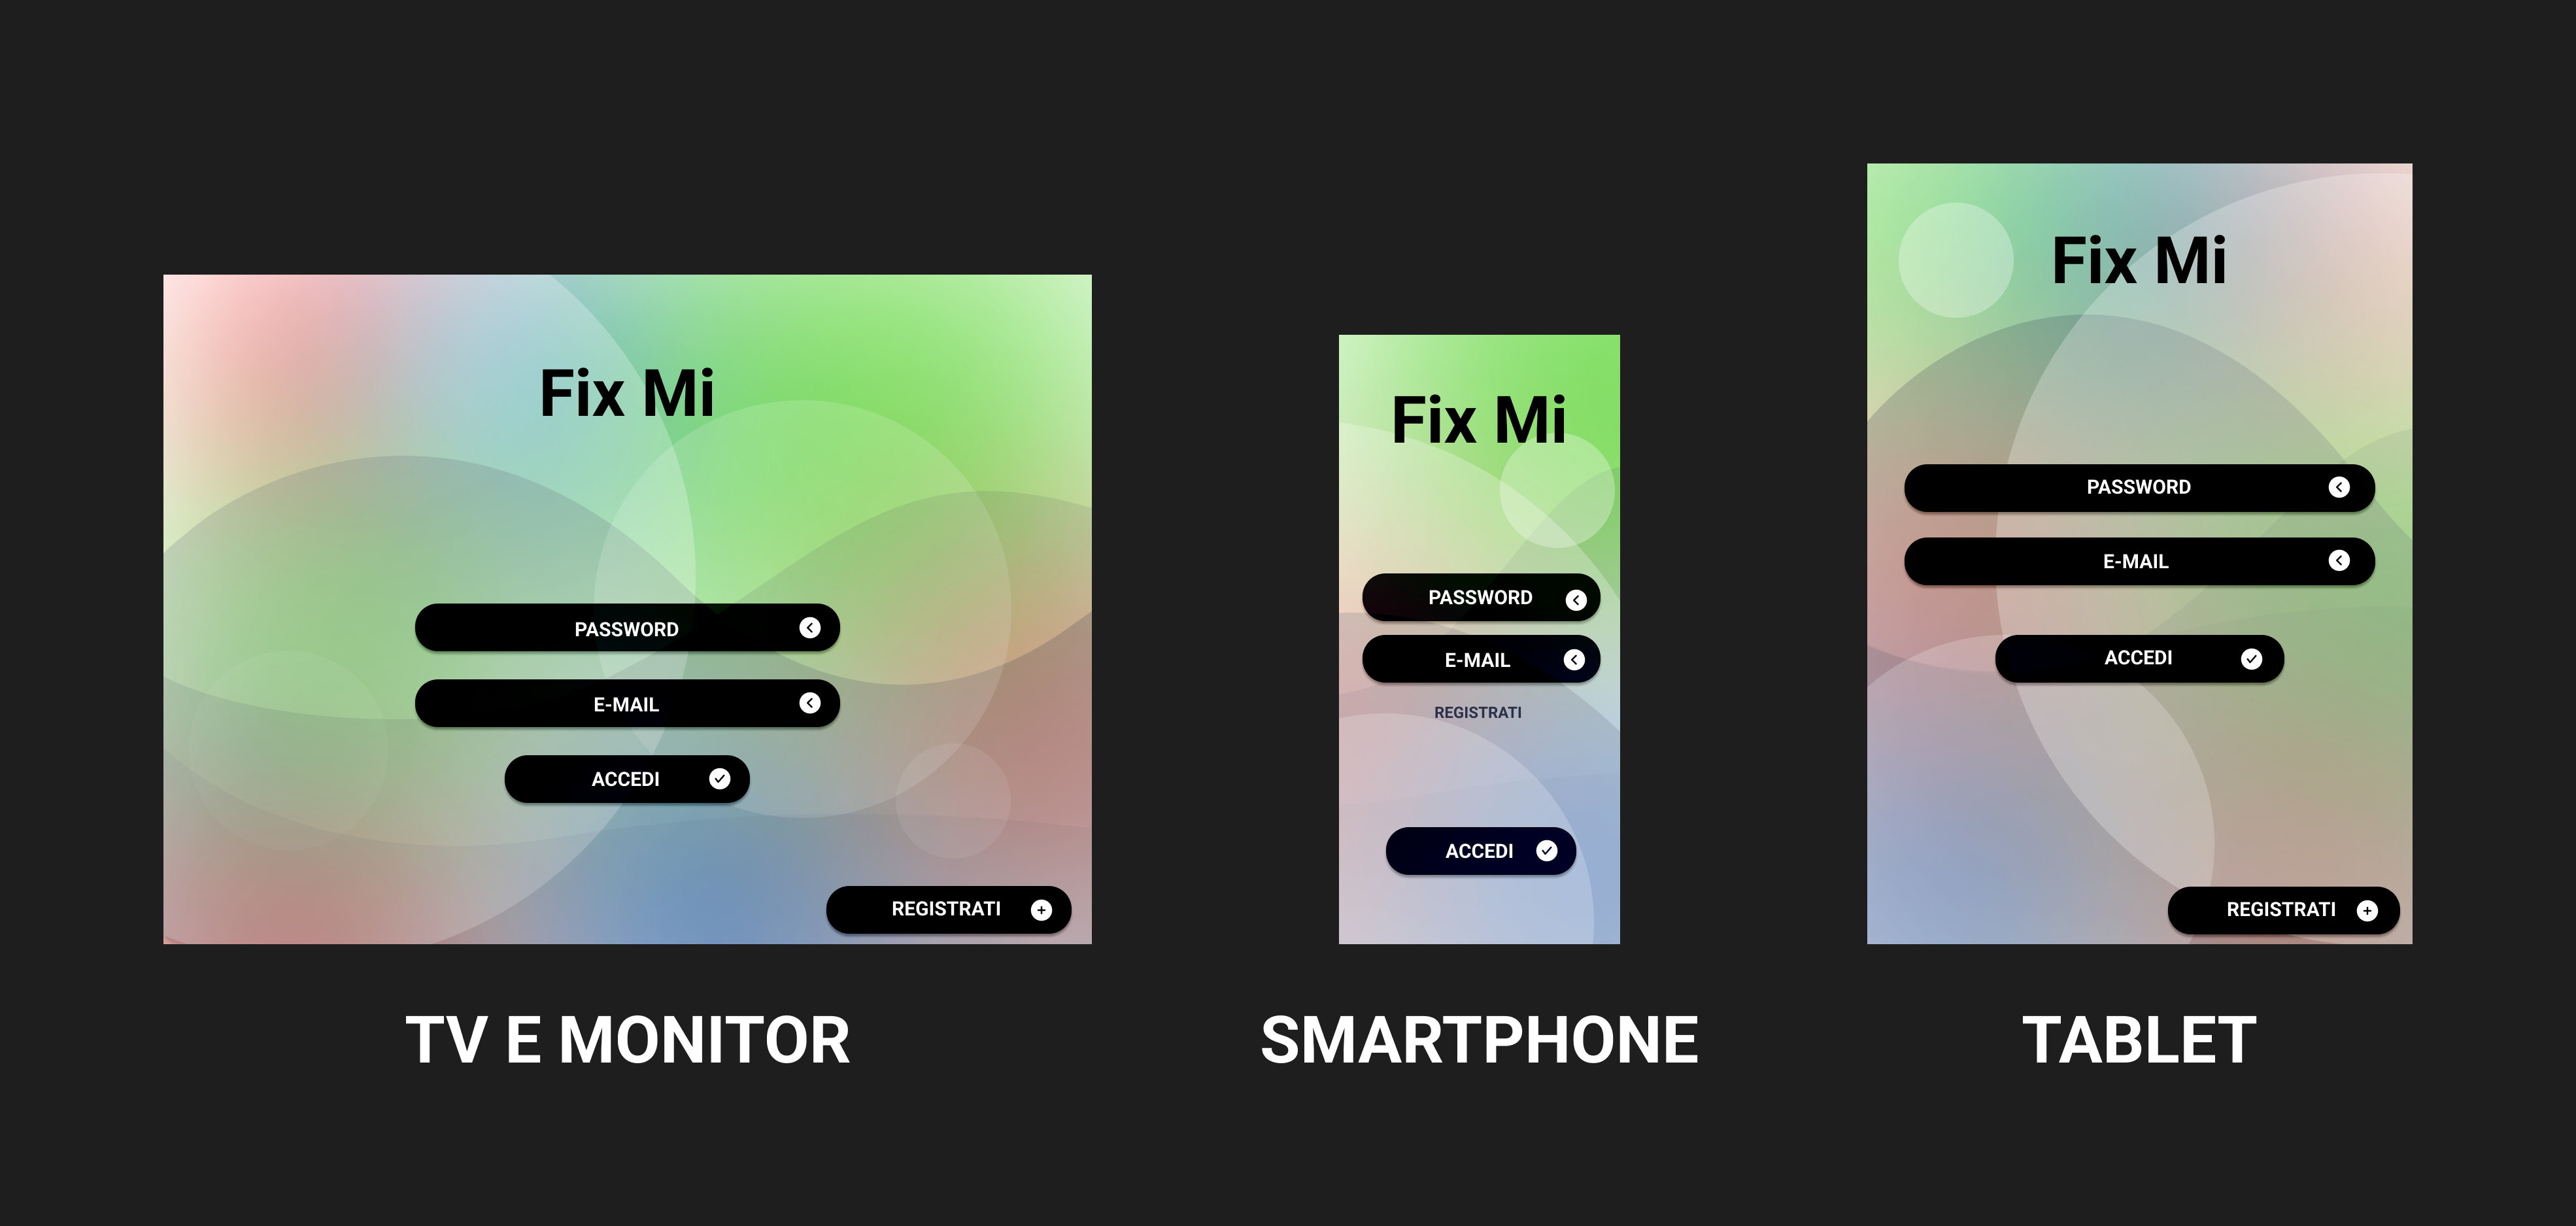
\includegraphics[width=1\textwidth]{images/Snapshots/login_snapshot.png}
	\caption{Schermata "Login" di "FixMi"}
\end{figure}	

\subsection*{Schermata Home}

La schermata "Home" permette di raggiungere tutte le aree principali del sistema attraverso appositi bottoni etichettati con il nome della suddetta area. In altro è presente una barra di navigazione, un bottone per accedere alle impostazioni ed uno per accedere al proprio profilo. In basso sono presenti le principali informazioni aziendali.

\begin{figure}[H]
	\centering
	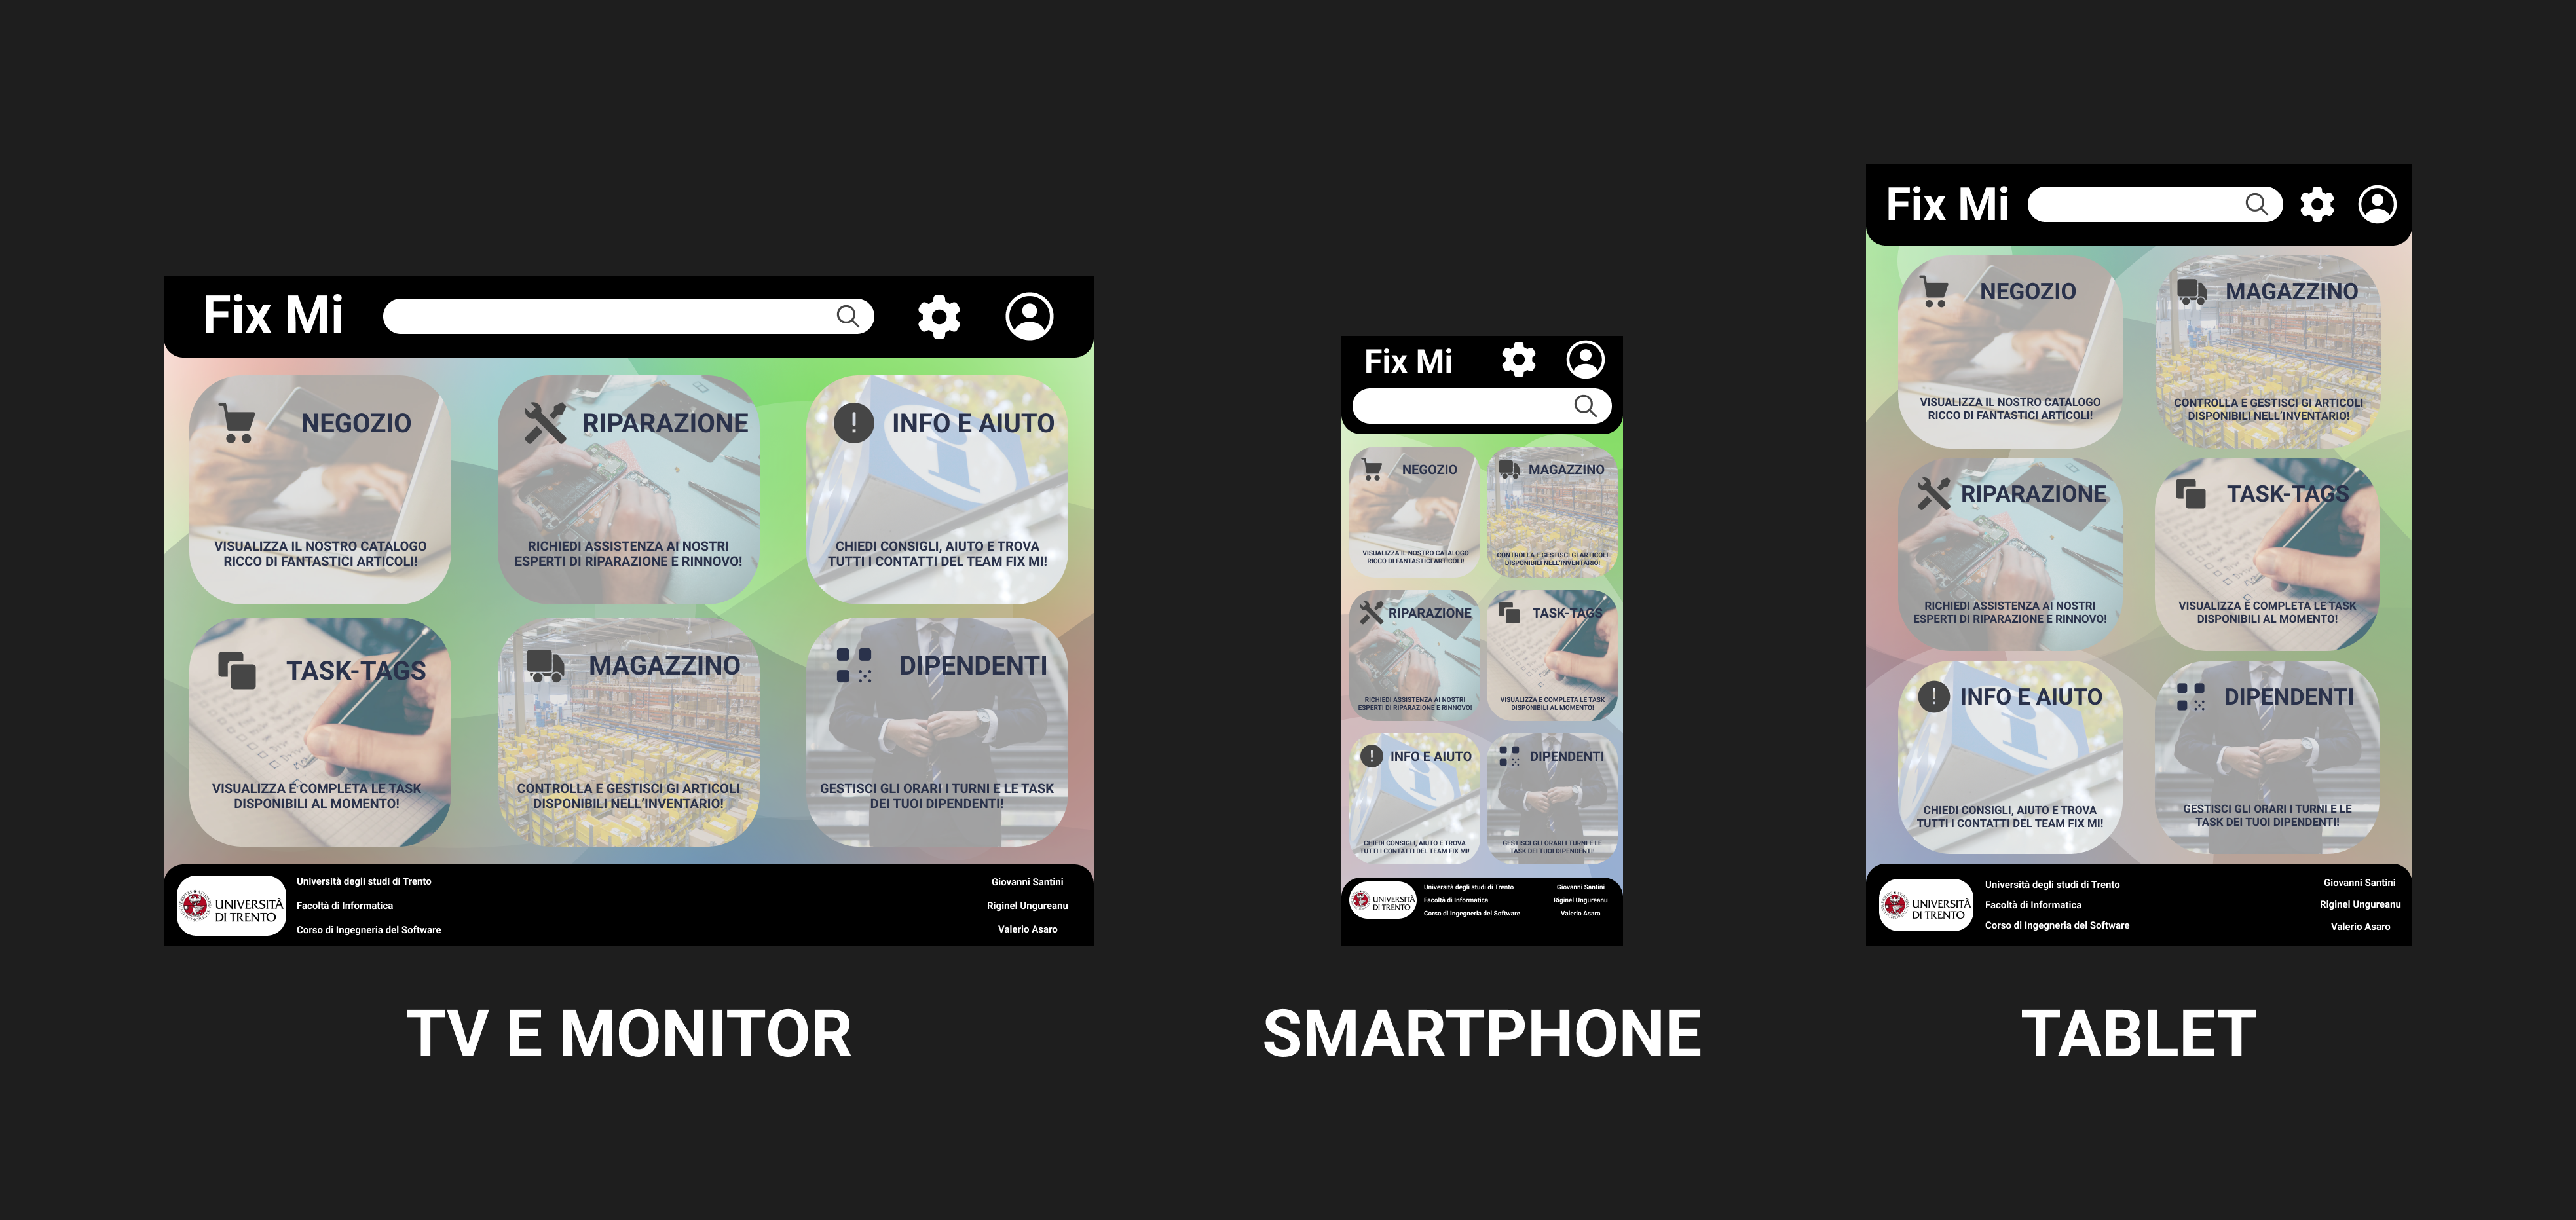
\includegraphics[width=1\textwidth]{images/Snapshots/mainpage_snapshot.png}
	\caption{Schermata "Home" di "FixMi"}
\end{figure}	

\subsection*{Schermata Magazzino}
La schermata "Magazzino" permette al Dipendente ed al Manager di poter gestire il catalogo aziendale. E' possibile fare una ricerca più accurata inserendo valide informazioni nei quattro campi presenti nella parte superiore della schermata.

\begin{figure}[H]
	\centering
	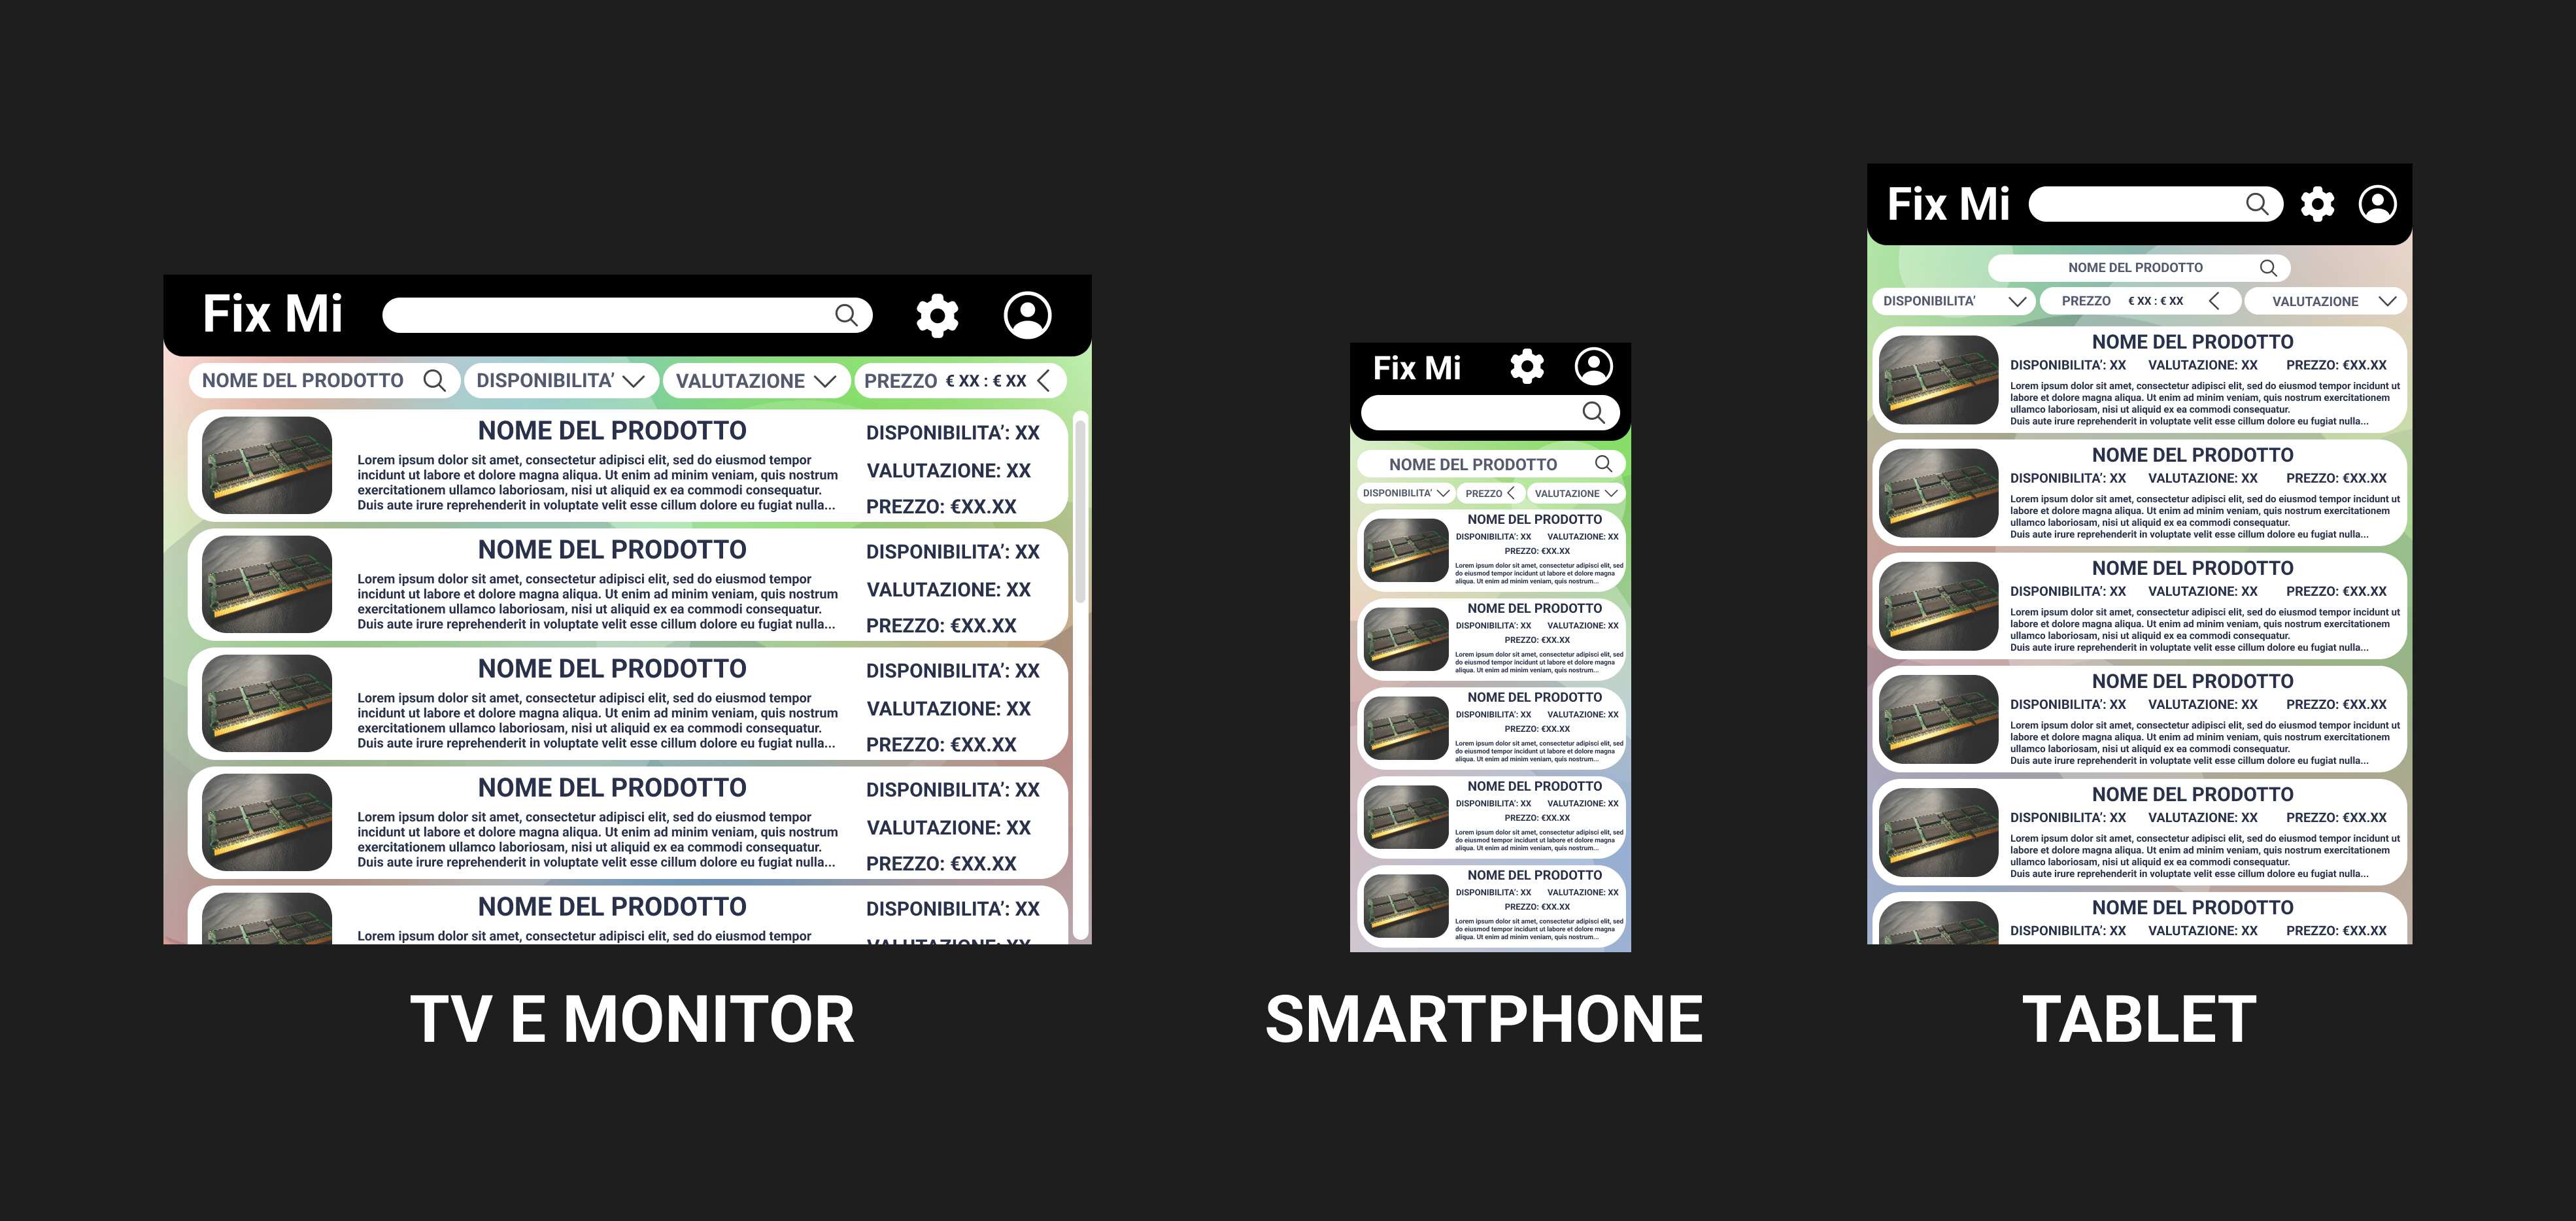
\includegraphics[width=1\textwidth]{images/Snapshots/magazzino_snapshot.png}
	\caption{Schermata "Magazzino" di "FixMi"}
\end{figure}	


\section{Design del Back-End}

Nella seguente sezione vengono riportate le specifiche generali per quanto riguarda la back-end dell’applicazione.

\subsection{Divisione in Microservizi}

La Back-End presenta un’architettura basata su microservizi indipendenti che comunicano tramite API. In particolare i microservizi sono:
\begin{itemize}
	\item Home
	\item Autenticazione
	\item Negozio
	\item Magazzino
	\item Task
	\item E-mail Server
	\item Gestione Dipendenti
\end{itemize}

\subsection{Sistemi Esterni}
L’applicazione si interfaccerà con i seguenti sistemi esterni:

\subsubsection{Sistemi di Pagamento}
La back-end si interfaccierà con "Paypal Name-Value-Pair" (NVP) e "NEXI XPay" per effettuare i pagamenti nella pagina "Negozio" (RF3). 

\subsubsection{Databases}
La Back-End utilizzerà il servizio "MongoDB Cluster Atlas" per interagire con databases distribuiti, in particolare i database per gli utenti registrati, le Task e il magazzino.

\subsubsection{OpenStreetMap}
Nella pagina di informazioni, l'applicazione userà OpenStreetMap per visualizzare la posizione dell'azienda nella mappa.

\subsubsection{2FA}
Il sito utilizzerà un servizio esterno per effettuare l'autenticazione a 2 fattori.

\subsection{Descrizione Microservizi}

\subsubsection*{Home}
Home presenta la pagina principale "Home" e permette di reinderizzare l'utente al microservizio desiderato tra Autenticazione, Negozio, Magazzino, Task, Gestione Dipendenti, in base al livello di autorizzazione, e alle pagine Feedback, Assistenza, Informazioni.

\subsubsection*{Autenticazione}
Il microservizio gestisce la registrazione e l'autenticazione degli utenti. Si interfaccia ad un database non relazionale esterno per memorizzare i profili e le rispettive informazioni.

\subsubsection*{Server E-mail}
L'applicazione prevede di implementare un server "SMTP" per l’invio delle e-mail a tutti i tipi di utente e prevede una e-mail aziendale per i dipendenti e per i manager.

\subsubsection*{Gestione delle Task}
Il microservizio si interfaccia con database esterno non relazionale per memorizzare le Task, mostrarle ai dipendenti e salvarne lo stato (definito nel capitolo 6).

\subsubsection*{Gestione dei Dipendenti}
Il microservizio è in grado di leggere e scrivere nel database delle Task e degli utenti registrati.

\subsubsection*{Magazzino}
Il microservizio utilizza un database non relazionale per memorizzare gli articoli contenuti all’interno del magazzino, oltre che alle operazioni svolte, come:

\begin{itemize}
	\item l’aggiunta di un nuovo articolo
	
	\item la rimozione di un articolo esistente
\end{itemize}

\subsection{Grafici}

In seguito uno schema di alto livello dei collegamenti tra i diversi microservizi. In blu i microservizi, in giallo i sistemi esterni, in verde le basi di dati.

\begin{figure}[H]
	%\centering
	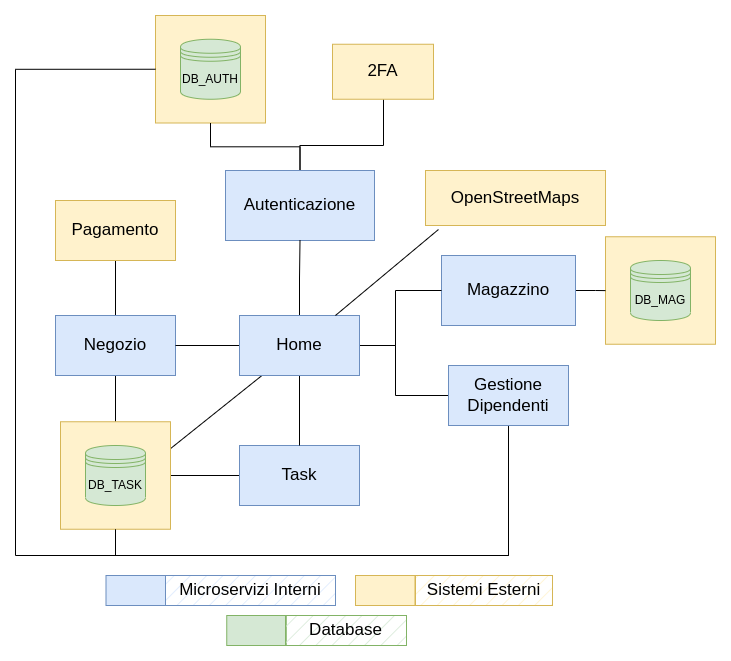
\includegraphics[width=1\textwidth]{images/back_end_short}
	\caption{Schema di alto livello della back-end}
\end{figure}	

% removed
\iffalse
\begin{figure}[H]
	\centering
	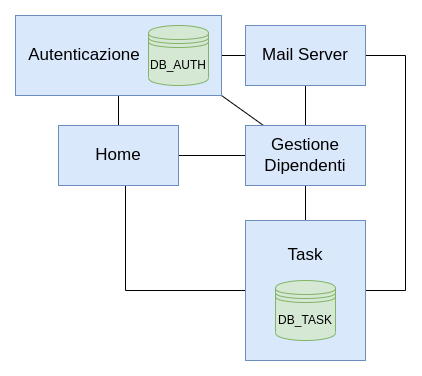
\includegraphics[width=0.4\textwidth]{images/admin_back_end}
	\caption{Gestione Dipendenti, disponibile solo per il manager}
\end{figure}

\begin{figure}[H]
	\centering
	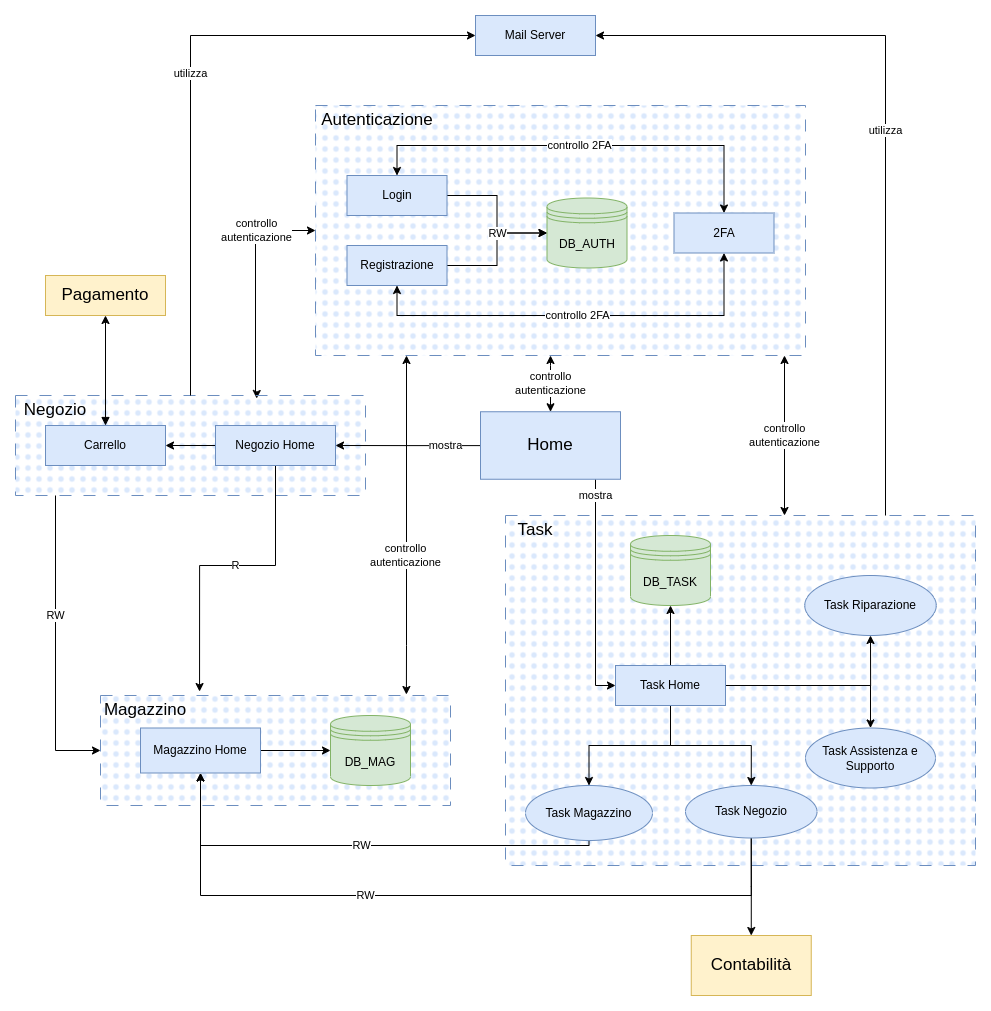
\includegraphics[width=1.1\textwidth]{images/backend_D1}
	\caption{Microservizi disponibili per tutti, con maggiore dettaglio}
\end{figure}
\fi


% -----------------------------

\chapter{Ruoli e Responsabilità}
Il team di sviluppo ha suddiviso l’obiettivo del progetto in obiettivi secondari di cui sono stati successivamente individuati ruoli e responsabilità:

% table
\begin{table}[!ht]
	\begin{center} % center the table
		\centering
		\begin{tabular}{ |p{5cm}|p{5cm}|  }
			\hline
			\centering Ruolo & \qquad\qquad\quad Membro \\ % I found no other way...
			\hline
			Sviluppo dell'obiettivo & Il gruppo di sviluppo \\
			\hline
			Leader del team di sviluppo & Riginel Ungureanu \\
			\hline
			Supervisore Back-End &
			Giovanni Santini \\
			\hline
			Supervisore Front-End & Valerio Asaro\\
			\hline
		\end{tabular}
		\caption{Relazione tra Ruoli e Membri}
	\end{center}
\end{table}

\chapter{Tecniche e Strumentazione}
Diversi strumenti e tecniche sono state scelte accuratamente in base alla situazione posta dall’obiettivo. Di seguito un elenco degli strumenti utilizzati per la realizzazione del progetto:

\begin{itemize}
	\item Trello \qquad \url{https://trello.com/}
	\item GitHub \qquad \url{https://github.com/}
	\item Google Suite \qquad \url{https://workspace.google.it/intl/it/}
	\item LaTeX \qquad \url{https://www.latex-project.org/}
	\item VSCode \qquad \url{https://code.visualstudio.com/}
	\item Figma \qquad \url{https://www.figma.com/}
	\item Coolors \qquad \url{https://coolors.co/}
	\item Diagrams \qquad \url{https://app.diagrams.net/}
	\item Vim \qquad \url{https://www.vim.org/}
\end{itemize}

\chapter{Glossario}
Segue la definizione dei principali termini utilizzati all'interno del documento:

\subsubsection*{2FA}
Il "2FA", in Italiano chiamato "Autenticazione a due fattori", è un metodo di autenticazione che consiste nel generare un codice temporaneo (Vedere "OTP") che solo l'utente in procinto di accedere conosce, aumentando notevolmente la sicurezza del sistema.
\subsubsection*{E-mail}
La "E-mail, anche chiamata "Posta Elettronica" è un sistema di comunicazione ampiamente utilizzato nel mondo odierno.
\subsubsection*{Microservizio}
Per Microservizio si intende una componente autosufficiente del sistema "FixMi" atta a svolgere uno specifico compito. L'unione di tutti i microservizi risulta essere di conseguenza il vero e proprio sistema "FixMi".
\subsubsection*{Front-End}
Con il termine "Front-End" si intende quella parte di sistema visibile all'utente ed a chiunque tenti di raggiungere il sito web.
\subsubsection*{Back-End}
Con il termine "Back-End", si riferisce a quella parte di sistema dedicata alla gestione dei dati e delle funzioni appartenenti al sito web.
\subsubsection*{OTP}
L'acronimo "OTP" sta per "One Time Password", è un codice generato temporaneamente e che viene mostrato solo all'utente, utilizzato per l'autenticazione a due fattori (Vedere "2FA").
\subsubsection*{Password}
Per "Password" si intende una serie di lettere, numeri e simboli conosciuti solo dall'utente. Potendo solo quest'ultimo sapere la corretta "Parola d'ordine" l'accesso al sistema risulta essere più sicuro e meno vulnerabile da attacchi informatici.
\subsubsection*{Task}
Il termine "Task", tradotto in Italiano "Compito" o "Mansione", viene utilizzato nel sistema "FixMi" per fissare gli obiettivi ed i traguardi che gli impiegati devono raggiungere.
\subsubsection*{Task-Tag}
Le "Task-Tag", cioè "Etichetta del Compito", servono a meglio definire l'ambito e la funzione in cui una determinata "Task" si trova (Vedere "Task").
\subsubsection*{Work-Tag}
Le "Work-Tag", "Etichette del Lavoro", vengono utilizzate per stabilire le diverse mansioni che un dipendente è in grado ed in dovere di svolgere. Diverse "Work-Tags" possono essere attribuite ad un singolo dipendente.


\end{document}